\documentclass[a4paper]{article}
\usepackage[T1]{fontenc}
\usepackage{fullpage}
\usepackage{graphicx}
\usepackage{url}

\usepackage{helvet}
\renewcommand{\familydefault}{\sfdefault}

%\usepackage[fontsize=18pt]{scrextend}
%\usepackage{setspace}
%\onehalfspacing

\newcommand{\file}[1]{\textsf{#1}}

\newcounter{saveFootnote}
\usepackage{fancybox}
\newcommand{\important}[1]{\setcounter{saveFootnote}{\value{footnote}}\vspace{0.3cm}\doublebox{\begin{minipage}{14.5cm}#1\end{minipage}}\vspace{0.3cm}}

\title{Réalisation du «net code» d'un jeu vidéo simple\\ Présentation du projet}
\author{Projet de programmation système (R3.05)\\ Année 2023-2024}
\date{loig.jezequel@univ-nantes.fr}

\begin{document}
\maketitle{}

\section{Objectif du projet}

Le code d'un jeu vidéo très simple, reprenant le principe du puissance 4, vous est fourni.
Dans la version actuelle de ce code, un joueur contrôle ses pions au clavier et les pions de l'autre sont contrôlés par un générateur de nombres aléatoires.
Votre objectif sera de permettre que les pions de ce second joueur soient contrôlés par une autre personne à travers le réseau.

\section{Description du jeu fourni}

Le jeu qui vous est fourni est un jeu de puissance 4.
Il se déroule en 4 étapes, qui sont décrites dans cette partie telles qu'elles fonctionnent actuellement.
Chacune de ces étapes devra être plus ou moins fortement modifiée au cours de ce projet pour permettre le jeu par le réseau.

Pour tester le jeu il suffit de récupérer le code fourni sur le Gitlab de l'Université et d'utiliser \verb|go build| dans le répertoire où se trouve le fichier \verb|go.mod|.
Ceci construit un exécutable \verb|course| qui permet de lancer le jeu.

\important{Attention, pour pouvoir utiliser la bibliothèque Ebitengine, qui est la base de ce projet, vous devez installer les paquets suivants sur votre machine virtuelle Ubuntu~: \file{libgl1-mesa-dev} et \file{xorg-dev}}

\subsection{Écran titre}

Au lancement du jeu, un écran titre s'affiche (figure~\ref{fig:titre}). Il suffit d'appuyer sur entrée pour passer à l'étape suivante.

\begin{figure}[htbp]
  \centering
  
\includegraphics[width=150pt]{titre.png}
  \caption{Écran d'accueil}\label{fig:titre}
\end{figure}

\subsection{Choix des couleurs}

La deuxième étape est la sélection d'une couleur pour les pions du joueur (figure~\ref{fig:selection}).
Le joueur peut sélectionner cette couleur à l'aide des flèches directionnelles puis valider son choix avec la touche entrée.
L'autre couleur est sélectionnée au hasard.

\begin{figure}[htbp]
  \centering
  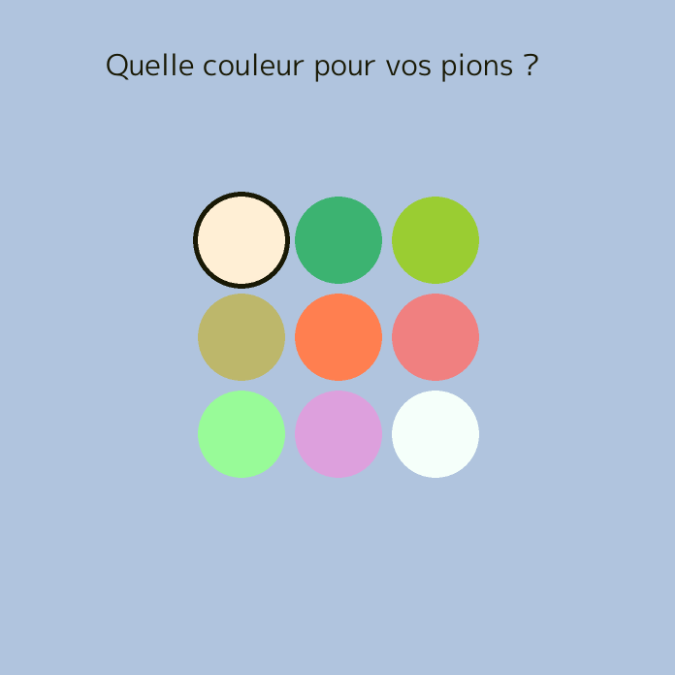
\includegraphics[width=150pt]{selection.png}
  \caption{Choix des personnages}\label{fig:selection}
\end{figure}

\subsection{Jeu !}

La troisième étape est la partie de puissance 4 en elle même (figure~\ref{fig:course}).
Le joueur contrôle les pions de la couleur qu'il a préalablement sélectionnée. 
Il peut choisir la colonne où jouer son prochain pion avec les touches gauche et droite.
Pour jouer un pion il faut appuyer sur bas (ou sur entrée).
Les pions de l'autre couleur sont contrôlés aléatoirement.
Une fois que quatre pions de la même couleur sont alignés ou que la grille est remplie, la partie se termine.

\begin{figure}[htbp]
  \centering
  
\includegraphics[width=150pt]{course.png}
  \caption{Course}\label{fig:course}
\end{figure}

\subsection{Résultats}

La dernière étape est celle des résultats.
Si le joueur a gagné (il a aligné 4 pions de sa couleur), perdu (4 pions de l'autre couleur ont été alignés), ou qu'il y a égalité (il n'y a pas 4 pions d'une même couleur alignés et la grille est pleine), cela s'affiche à l'écran.
Après cela, le joueur peut appuyer sur entrée pour redémarrer une partie (retour à l'étape du jeu, le perdant de la partie précédante commence).

\begin{figure}[htbp]
  \centering
  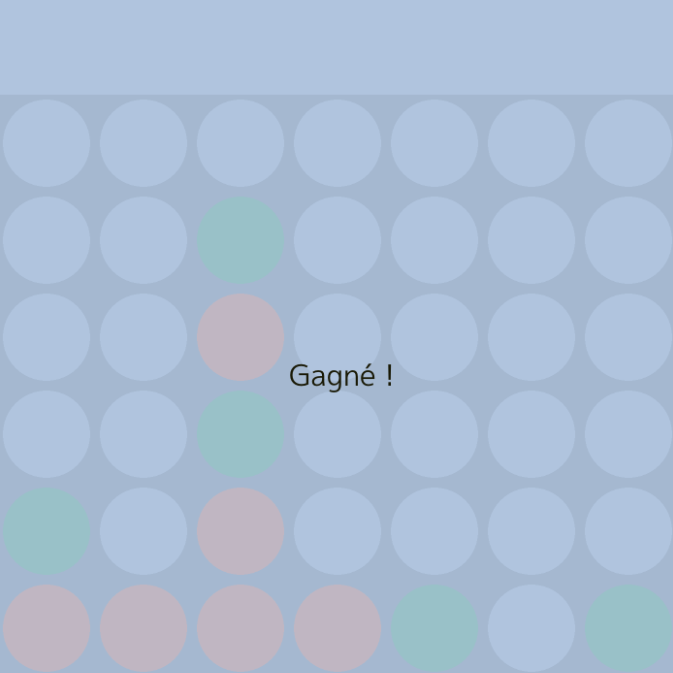
\includegraphics[width=150pt]{results.png}
  \caption{Résultats}\label{fig:resultats}
\end{figure}

\section{Description du jeu attendu}
\label{section:todo}

Il vous faudra modifier le code fourni afin de permettre à deux joueurs de contrôler chacun une couleur de pions et de jouer ensemble à travers le réseau.
Le principe sera que chaque joueur démarre le jeu sur sa machine (en indiquant l'adresse d'un serveur) et contrôle une couleur de pions (en tant que joueur 1 sur son instance du jeu).
Par contre, au lieu d'être contrôlés aléatoirement, les pions du joueur 2 (de chaque instance) reflètent les choix de l'autre joueur.
Ceci implique que le jeu de chaque joueur retransmette à destination de l'autre jeu, via un serveur, des informations sur ce que fait ce joueur.

\section{Ce que vous aurez à faire}

Pour obtenir la moyenne, il vous faut écrire un code Go qui réponde, au minimum, à la demande exprimée dans les différents sujets qui vous seront distribués au cours de ce projet.
Ce code reposera sur le code qui vous est fourni.

Pour nous faciliter la correction, il faudra identifier au mieux votre contribution~:
\begin{itemize}
  \item les nouvelles fonctions seront écrites dans des nouveaux fichiers,
  \item les modifications à mes fonctions seront clairement indiquées par des commentaires.
\end{itemize}
Votre code devra bien sûr être commenté pour indiquer l'utilité de chacune de vos fonctions (sur le modèle du code fourni) et, si besoin, décrire l'implémentation des plus complexes d'entre elles.

Pour obtenir une note supérieure à la moyenne il vous faudra ajouter des améliorations, parmi celles qui vous seront suggérées au cours du projet (plus vous en ajoutez, plus votre note sera élevée).

En plus du bon fonctionnement de votre programme, la qualité de votre code et de vos commentaires pourront bien sûr aussi améliorer ou réduire votre note. Du moment que le jeu tourne toujours de manière fluide (i.e. aux alentours de 60 frames par seconde) les performances de votre code ne seront par contre pas prises en compte de manière négative.

\section{Hypothèses simplificatrices}

Pour simplifier l'implémentation on considérera les hypothèses suivantes.

\begin{itemize}
\item Aucun joueur n'est déconnecté durant toute la durée du jeu.
\item Il y a un faible délai entre l'émission et la réception d'un message à travers le réseau.
\item Aucun message envoyé sur le réseau n'est perdu.
\item Les messages arrivent dans l'ordre où ils ont été émis (si m1 puis m2 sont envoyés par un programme p1 à destination d'un programme p2, alors p2 recevra toujours m1 avant m2).
\end{itemize}

\end{document}
